This appendix presents the comprehensive benchmark evaluation statistics across all 16 evaluated architectural configurations ($C_0$--$C_{15}$) on the original, unconstrained raw enterprise knowledge corpus.

\begin{table}[htbp]
\centering
\small
\setlength{\tabcolsep}{3.5pt}
\caption{End-to-end execution latency and Time-to-First-Token (TTFT) across 16 pipeline configurations on Enterprise. Statistical significance flags denote Holm-Bonferroni-adjusted paired Wilcoxon signed-rank tests against the naive baseline ($C_0$).}
\label{tab:latency_enterprise_raw}
\begin{tabular*}{\linewidth}{@{\extracolsep{\fill}} l l r r r r r @{}}
\toprule
\textbf{Config} & \textbf{Pipeline} & \makecell{\textbf{TTFT $P_{50}$}\\\scriptsize{(ms)}} & \makecell{\textbf{TTFT $P_{95}$}\\\scriptsize{(ms)}} & \makecell{\textbf{$T_{\text{total}} P_{50}$}\\\scriptsize{(ms)}} & \makecell{\textbf{$T_{\text{total}} P_{95}$}\\\scriptsize{(ms)}} & \makecell{\textbf{$\Delta T_{\text{total}}$}\\\scriptsize{(\%)}} \\
\midrule
\multicolumn{7}{l}{\textbf{Baseline ($k=0$)}} \\
$C_{0}$ & Naive RAG Baseline & 3953.5 & 16945.6 & 5175.5 & 25615.2 & -- \\
\midrule
\multicolumn{7}{l}{\textbf{Single-Factor Isolated ($k=1$)}} \\
$C_{1}$ & S2B & 7035.5 & 36325.2 & 8071.0 & 37151.1 & +55.9\%\textsuperscript{ns} \\
$C_{2}$ & SR & 2717.0 & 13192.0 & 3760.0 & 12919.3 & -27.4\%\textsuperscript{ns} \\
$C_{3}$ & PC & 3358.0 & 5014.0 & 6944.5 & 10861.9 & +34.2\%\textsuperscript{ns} \\
$C_{4}$ & MC & 2191.0 & 6490.0 & 2319.0 & 7539.6 & -55.2\%\textsuperscript{ns} \\
\midrule
\multicolumn{7}{l}{\textbf{Pairwise Combinations ($k=2$)}} \\
$C_{5}$ & S2B + SR & 2418.5 & 4987.0 & 4205.5 & 5484.1 & -18.7\%\textsuperscript{ns} \\
$C_{6}$ & S2B + PC & 8609.5 & 28373.8 & 15526.0 & 30194.5 & +200.0\%\textsuperscript{ns} \\
$C_{7}$ & S2B + MC & 2577.5 & 14474.0 & 3864.0 & 14564.3 & -25.3\%\textsuperscript{ns} \\
$C_{8}$ & SR + PC & 6315.5 & 35144.8 & 10090.0 & 40675.9 & +95.0\%\textsuperscript{ns} \\
$C_{9}$ & SR + MC & 2561.5 & 12484.8 & 3019.5 & 12928.9 & -41.7\%\textsuperscript{ns} \\
$C_{10}$ & PC + MC & 4224.0 & 9722.7 & 6524.0 & 11593.9 & +26.1\%\textsuperscript{ns} \\
\midrule
\multicolumn{7}{l}{\textbf{Higher-Order Triplets \& Full-Stack ($k \ge 3$)}} \\
$C_{11}$ & S2B + SR + PC & 6429.0 & 12382.6 & 10774.5 & 17835.3 & +108.2\%\textsuperscript{ns} \\
$C_{12}$ & S2B + SR + MC & 2986.5 & 4379.9 & 3796.5 & 5590.1 & -26.6\%\textsuperscript{ns} \\
$C_{13}$ & S2B + PC + MC & 4823.0 & 9698.7 & 7396.0 & 14923.6 & +42.9\%\textsuperscript{ns} \\
$C_{14}$ & SR + PC + MC & 5996.5 & 69574.2 & 11373.5 & 72518.0 & +119.8\%\textsuperscript{ns} \\
$C_{15}$ & S2B + SR + PC + MC (Full-Stack) & 3336.0 & 116262.0 & 6257.0 & 118083.8 & +20.9\%\textsuperscript{ns} \\
\bottomrule
\end{tabular*}
\vspace{0.5em}
\parbox{\linewidth}{\footnotesize
\textbf{Notes:} $P_{50}$ and $P_{95}$ denote median and 95th percentile execution latencies. TTFT denotes Time-to-First-Token. $\Delta T_{\text{total}}$ reflects percentage change in median latency relative to baseline ($C_0$). Statistical significance flags denote two-tailed paired Wilcoxon signed-rank tests against baseline ($C_0$) with Holm-Bonferroni correction ($^{*} p < 0.05$, $^{**} p < 0.01$, $^{***} p < 0.001$, $\mathrm{ns} = p \ge 0.05$).}
\end{table}


\begin{figure}[!htbp]
\centering
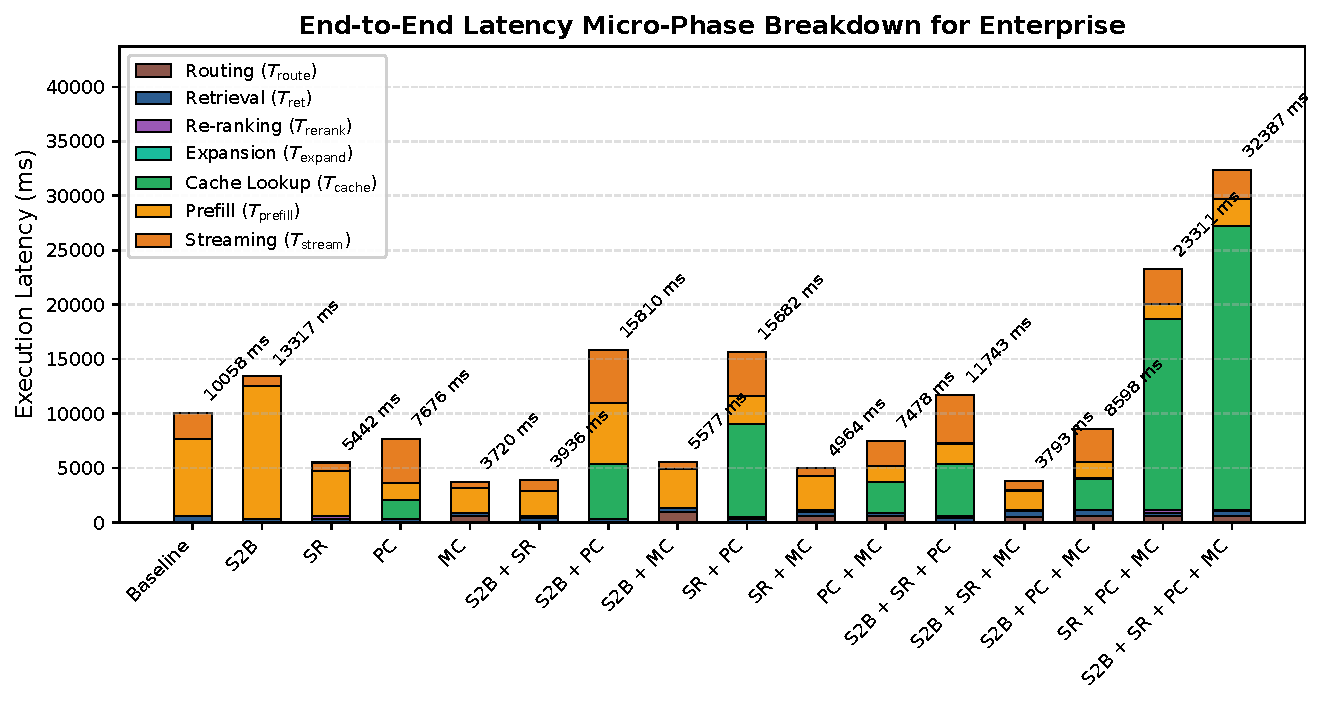
\includegraphics[width=\linewidth]{figures/enterprise/latency_breakdown_enterprise.pdf}
\caption{Component-wise latency breakdown across all 16 pipeline configurations on the unconstrained raw enterprise corpus, detailing execution duration across retrieval, semantic re-ranking, cache management, and model tier generation phases.}
\label{fig:latency_breakdown_enterprise_raw}
\end{figure}

\begin{table}[htbp]
\centering
\small
\setlength{\tabcolsep}{3.5pt}
\caption{Operational cost and token consumption breakdown across 16 pipeline architectures on Enterprise. Statistical significance flags denote Holm-Bonferroni-adjusted paired Wilcoxon signed-rank tests against the naive baseline.}
\label{tab:cost_enterprise_raw}
\begin{tabular*}{\linewidth}{@{\extracolsep{\fill}} l r r r r r @{}}
\toprule
\textbf{Pipeline} & \makecell{\textbf{Uncached}\\\textbf{Prompt Tok}} & \makecell{\textbf{Cached}\\\textbf{Prompt Tok}} & \makecell{\textbf{Output}\\\textbf{Tokens}} & \makecell{\textbf{Cost / 1k}\\\scriptsize{(\$)}} & \makecell{\textbf{$\Delta$ Cost}\\\scriptsize{(\%)}} \\
\midrule
\multicolumn{6}{@{}l@{}}{\textbf{Baseline ($k=0$)}} \\
Naive RAG Baseline & 5,646 & 812 & 218 & \$5.662 & -- \\
\midrule
\multicolumn{6}{@{}l@{}}{\textbf{Single-Factor Isolated ($k=1$)}} \\
S2B & 7,525 & 0 & 190 & \$6.355 & +12.2\%\textsuperscript{ns} \\
SR & 5,852 & 0 & 168 & \$10.020 & +77.0\%\textsuperscript{*} \\
PC & 33 & 0 & 584 & \$6.817 & +20.4\%\textsuperscript{*} \\
MC & 6,458 & 0 & 163 & \$3.887 & -31.3\%\textsuperscript{ns} \\
\midrule
\multicolumn{6}{@{}l@{}}{\textbf{Pairwise Combinations ($k=2$)}} \\
S2B + SR & 7,895 & 0 & 226 & \$11.771 & +107.9\%\textsuperscript{*} \\
S2B + PC & 28 & 0 & 428 & \$7.027 & +24.1\%\textsuperscript{ns} \\
S2B + MC & 7,525 & 0 & 173 & \$5.005 & -11.6\%\textsuperscript{ns} \\
SR + PC & 26 & 0 & 380 & \$11.073 & +95.6\%\textsuperscript{*} \\
SR + MC & 5,457 & 392 & 141 & \$8.436 & +49.0\%\textsuperscript{ns} \\
PC + MC & 24 & 0 & 323 & \$4.488 & -20.7\%\textsuperscript{ns} \\
\midrule
\multicolumn{6}{@{}l@{}}{\textbf{Higher-Order Combinations ($k \ge 3$)}} \\
S2B + SR + PC & 23 & 0 & 396 & \$12.181 & +115.1\%\textsuperscript{*} \\
S2B + SR + MC & 7,081 & 814 & 160 & \$9.638 & +70.2\%\textsuperscript{ns} \\
S2B + PC + MC & 28 & 0 & 463 & \$5.070 & -10.5\%\textsuperscript{ns} \\
SR + PC + MC & 26 & 0 & 477 & \$9.698 & +71.3\%\textsuperscript{ns} \\
S2B + SR + PC + MC & 23 & 0 & 440 & \$8.605 & +52.0\%\textsuperscript{ns} \\
\bottomrule
\end{tabular*}
\vspace{0.5em}
\parbox{\linewidth}{\footnotesize
\textbf{Notes:} Prompt and completion tokens represent query sample averages. If cached prompt tokens are reported ($N_{\text{cached}} > 0$), uncached prompt tokens are computed as $\max(0, N_{\text{prompt}} - N_{\text{cached}})$. Cost reflects Google Cloud Gemini Enterprise platform pricing normalized per 1,000 queries. $\Delta\text{Cost}$ reflects percentage change relative to the naive baseline. Statistical significance flags denote two-tailed paired Wilcoxon signed-rank tests against the naive baseline with Holm-Bonferroni correction ($^{*} p < 0.05$, $^{**} p < 0.01$, $^{***} p < 0.001$, $\mathrm{ns} = p \ge 0.05$).}
\end{table}


\begin{figure}[!htbp]
\centering
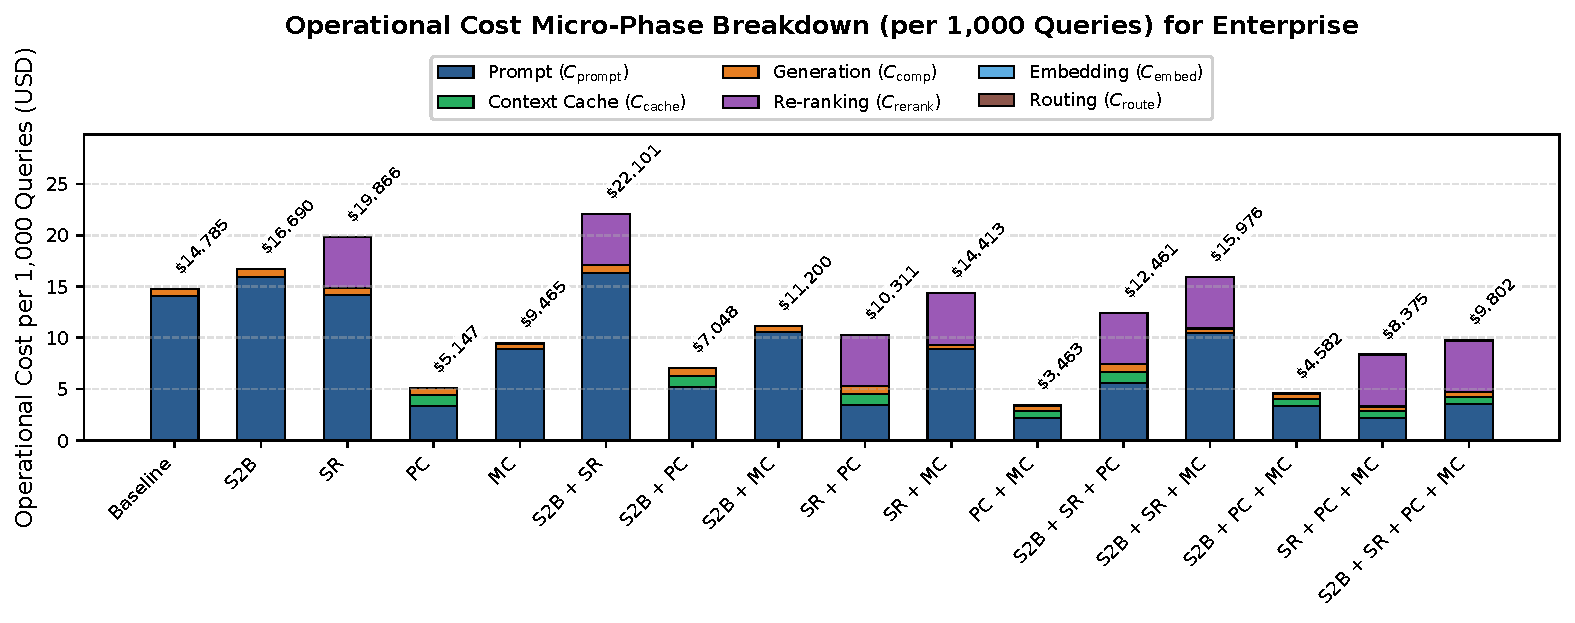
\includegraphics[width=\linewidth]{figures/enterprise/cost_breakdown_enterprise.pdf}
\caption{Component-wise operational expenditure breakdown per 1,000 queries across all 16 pipeline configurations on the unconstrained raw enterprise corpus, detailing monetary expenditure across uncached context prefill, context cache lookups, generative completion, and auxiliary neural re-ranking services.}
\label{fig:cost_breakdown_enterprise_raw}
\end{figure}

\begin{table}[htbp]
\centering
\scriptsize
\setlength{\tabcolsep}{2.2pt}
\caption{Retrieval, generation, and out-of-domain rejection quality metrics across 16 pipeline configurations on the Enterprise Knowledge Corpus ($N = 100$). Statistical significance flags denote Holm-Bonferroni-adjusted paired Wilcoxon signed-rank tests against the naive baseline ($C_0$).}
\label{tab:quality_enterprise}
\begin{tabular*}{\linewidth}{@{\extracolsep{\fill}} l l c c c c c c @{}}
\toprule
\textbf{Config} & \textbf{Pipeline} & \makecell{\textbf{Context}\\\textbf{Precision}} & \makecell{\textbf{Context}\\\textbf{Recall}} & \makecell{\textbf{Faithful-}\\\textbf{ness}} & \makecell{\textbf{Answer}\\\textbf{Relevancy}} & \makecell{\textbf{Refusal Acc. /}\\\textbf{FRR (\%)}} & \makecell{\textbf{Composite}\\\textbf{Quality $Q$}} \\
\midrule
\multicolumn{8}{l}{\textbf{Baseline ($k=0$)}} \\
$C_{0}$ & Naive RAG Baseline & 0.833 & 0.938 & 0.915 & 0.000 & 100.0\% / 0.0\% & \textbf{0.0004} \\
\midrule
\multicolumn{8}{l}{\textbf{Single-Factor Isolated ($k=1$)}} \\
$C_{1}$ & S2B & 0.955 & 0.875 & 0.953 & 0.000 & 100.0\% / 0.0\% & \textbf{0.0004}\textsuperscript{ns} \\
$C_{2}$ & SR & 0.869 & 0.938 & 0.975 & 0.000 & 100.0\% / 0.0\% & \textbf{0.0004}\textsuperscript{ns} \\
$C_{3}$ & PC & 0.854 & 0.938 & 0.492 & 0.000 & 0.0\% / 0.0\% & \textbf{0.0004}\textsuperscript{ns} \\
$C_{4}$ & MC & 0.854 & 0.938 & 0.894 & 0.000 & 100.0\% / 0.0\% & \textbf{0.0004}\textsuperscript{ns} \\
\midrule
\multicolumn{8}{l}{\textbf{Pairwise Combinations ($k=2$)}} \\
$C_{5}$ & S2B + SR & 0.886 & 0.812 & 0.934 & 0.000 & 100.0\% / 0.0\% & \textbf{0.0004}\textsuperscript{ns} \\
$C_{6}$ & S2B + PC & 0.962 & 0.875 & 0.360 & 0.000 & 0.0\% / 0.0\% & \textbf{0.0004}\textsuperscript{ns} \\
$C_{7}$ & S2B + MC & 1.000 & 0.938 & 0.951 & 0.000 & 100.0\% / 0.0\% & \textbf{0.0004}\textsuperscript{ns} \\
$C_{8}$ & SR + PC & 0.844 & 0.938 & 0.353 & 0.000 & 0.0\% / 0.0\% & \textbf{0.0004}\textsuperscript{ns} \\
$C_{9}$ & SR + MC & 0.869 & 0.938 & 0.840 & 0.000 & 100.0\% / 0.0\% & \textbf{0.0004}\textsuperscript{ns} \\
$C_{10}$ & PC + MC & 0.856 & 0.938 & 0.362 & 0.000 & 0.0\% / 0.0\% & \textbf{0.0004}\textsuperscript{ns} \\
\midrule
\multicolumn{8}{l}{\textbf{Higher-Order Triplets \& Full-Stack ($k \ge 3$)}} \\
$C_{11}$ & S2B + SR + PC & 0.865 & 0.812 & 0.602 & 0.000 & 0.0\% / 0.0\% & \textbf{0.0004}\textsuperscript{ns} \\
$C_{12}$ & S2B + SR + MC & 0.886 & 0.812 & 0.944 & 0.000 & 100.0\% / 0.0\% & \textbf{0.0004}\textsuperscript{ns} \\
$C_{13}$ & S2B + PC + MC & 0.962 & 0.938 & 0.376 & 0.000 & 0.0\% / 0.0\% & \textbf{0.0004}\textsuperscript{ns} \\
$C_{14}$ & SR + PC + MC & 0.879 & 1.000 & 0.454 & 0.000 & 0.0\% / 0.0\% & \textbf{0.0004}\textsuperscript{ns} \\
$C_{15}$ & S2B + SR + PC + MC (Full-Stack) & 0.765 & 0.833 & 0.261 & 0.000 & 0.0\% / 0.0\% & \textbf{0.0004}\textsuperscript{ns} \\
\bottomrule
\end{tabular*}
\vspace{0.5em}
\parbox{\linewidth}{\footnotesize
\textbf{Notes:} Context Precision, Context Recall, Faithfulness, and Answer Relevancy are evaluated via RAGAS~\citep{es2024ragas} exclusively on answerable queries. Refusal Accuracy evaluates correct abstention on unanswerable out-of-domain (OOD) queries, while False Refusal Rate (FRR) measures erroneous abstention on answerable queries. Composite Quality $Q \in [0, 1]$ represents the regularized harmonic mean across the four RAGAS dimensions on answerable queries (Equation~\ref{eq:composite_quality}, $\epsilon = 10^{-4}$). Statistical significance flags denote two-tailed paired Wilcoxon signed-rank tests against baseline ($C_0$) with Holm-Bonferroni correction ($^{*} p < 0.05$, $^{**} p < 0.01$, $^{***} p < 0.001$, $\mathrm{ns} = p \ge 0.05$).}
\end{table}


\begin{figure}[!htbp]
\centering
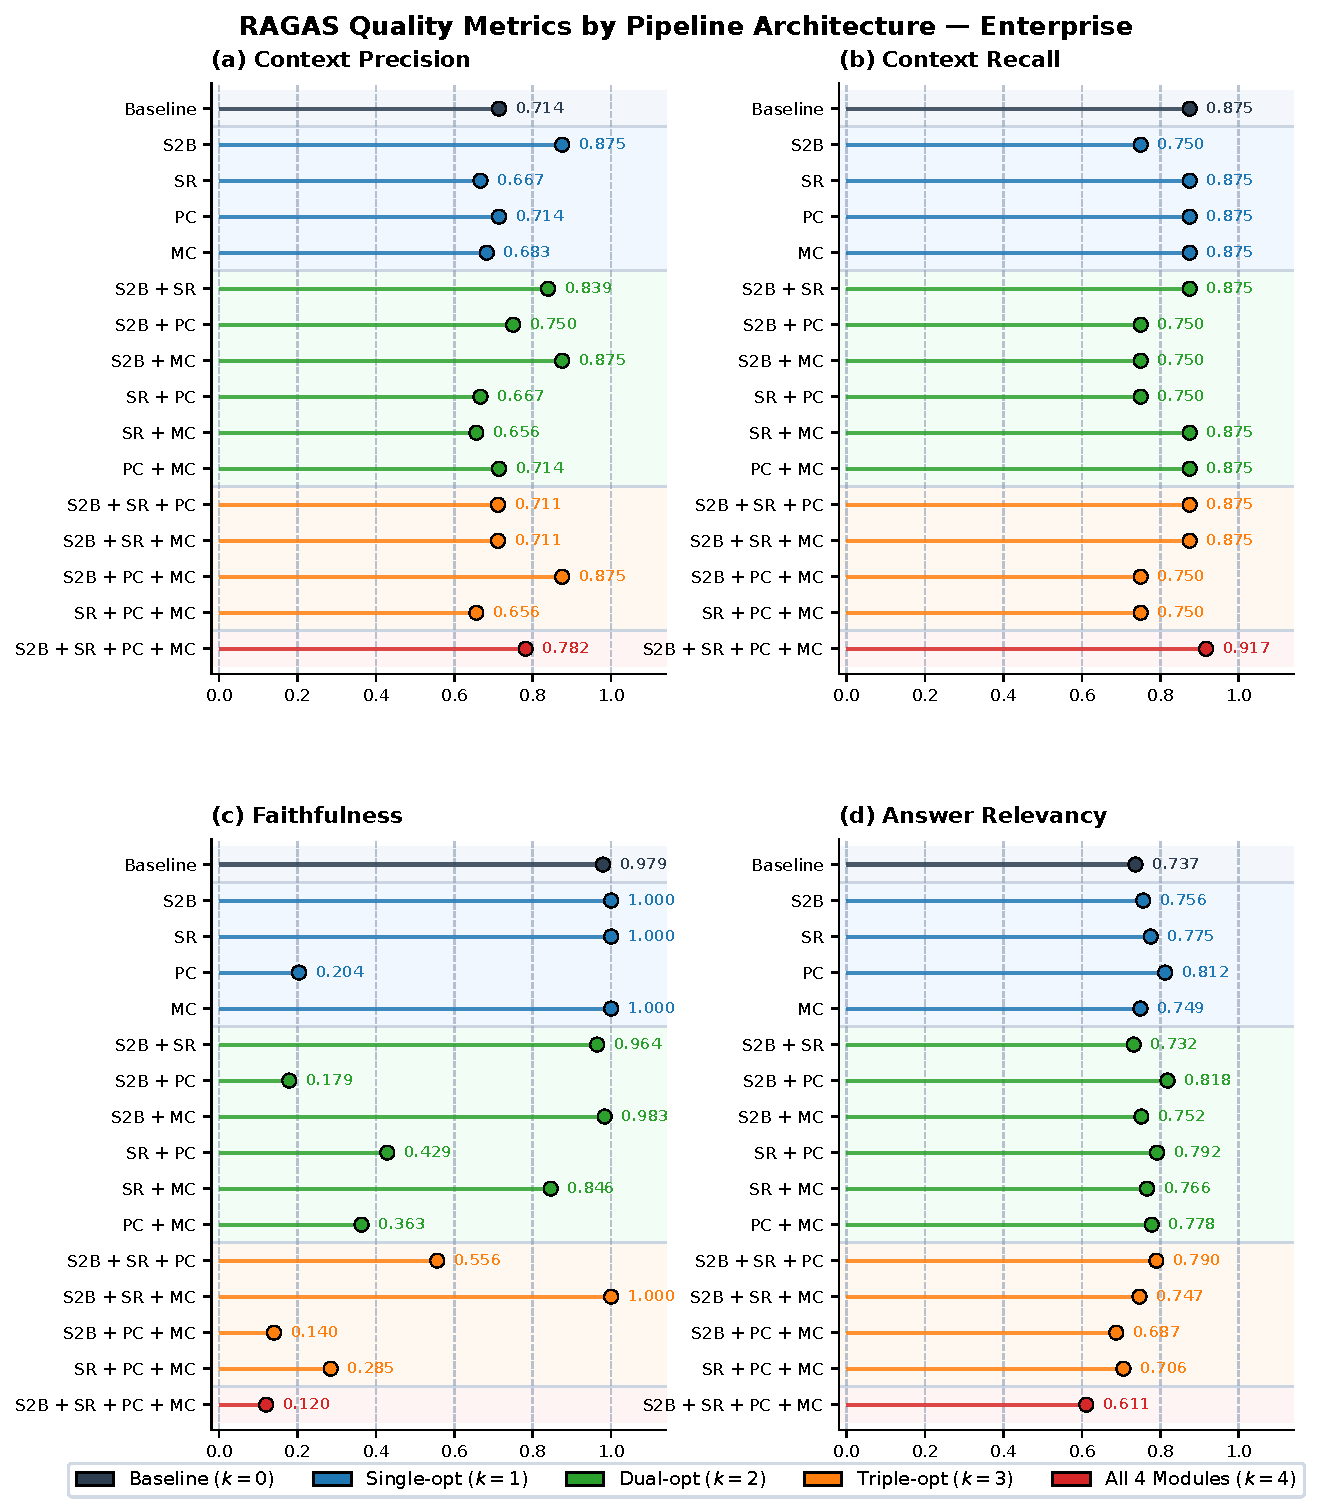
\includegraphics[width=\linewidth]{figures/enterprise/quality_lollipop_enterprise.pdf}
\caption{Multi-dimensional response quality profiles across architectural configurations on the unconstrained raw enterprise corpus, comparing Context Precision, Context Recall, Faithfulness, and Answer Relevancy across architectural tiers ($C_0$--$C_{15}$). Horizontal lollipop plots with tier-stratified background shading isolate configuration-level variations.}
\label{fig:quality_lollipop_enterprise_raw}
\end{figure}

\begin{table}[htbp]
\centering
\small
\setlength{\tabcolsep}{3.5pt}
\caption{Multi-objective Pareto efficiency and 3D non-domination trade-off metrics across 16 pipeline architectures on Enterprise.}
\label{tab:pareto_enterprise_raw}
\begin{tabular*}{\linewidth}{@{\extracolsep{\fill}} l c r r r r c @{}}
\toprule
\textbf{Pipeline} & \makecell{\textbf{Composite}\\\textbf{Quality $Q$}} & \makecell{\textbf{Cost / 1k}\\\scriptsize{(\$)}} & \makecell{\textbf{$T_{\text{total}} P_{50}$}\\\scriptsize{(s)}} & \textbf{QPD} & \textbf{QPS} & \makecell{\textbf{Pareto}\\\textbf{Optimal}} \\
\midrule
\multicolumn{7}{@{}l@{}}{\textbf{Baseline ($k=0$)}} \\
Naive RAG Baseline & 0.7165 & \$5.662 & 5.18 & 127 & 0.07 & No \\
\midrule
\multicolumn{7}{@{}l@{}}{\textbf{Single-Factor Isolated ($k=1$)}} \\
S2B & 0.7472 & \$6.355 & 8.07 & 118 & 0.06 & \textbf{Yes} \\
SR & 0.6515 & \$10.020 & 3.76 & 65 & 0.12 & No \\
PC & 0.4501 & \$6.817 & 6.94 & 66 & 0.06 & No \\
MC & 0.6994 & \$3.887 & 2.32 & 180 & 0.19 & \textbf{Yes} \\
\midrule
\multicolumn{7}{@{}l@{}}{\textbf{Pairwise Combinations ($k=2$)}} \\
S2B + SR & 0.8136 & \$11.771 & 4.21 & 69 & 0.21 & \textbf{Yes} \\
S2B + PC & 0.2981 & \$7.027 & 15.53 & 42 & 0.02 & No \\
S2B + MC & 0.7254 & \$5.005 & 3.86 & 145 & 0.13 & \textbf{Yes} \\
SR + PC & 0.4589 & \$11.073 & 10.09 & 41 & 0.03 & No \\
SR + MC & 0.5179 & \$8.436 & 3.02 & 61 & 0.10 & No \\
PC + MC & 0.3300 & \$4.488 & 6.52 & 74 & 0.04 & No \\
\midrule
\multicolumn{7}{@{}l@{}}{\textbf{Higher-Order Combinations ($k \ge 3$)}} \\
S2B + SR + PC & 0.5186 & \$12.181 & 10.77 & 43 & 0.04 & No \\
S2B + SR + MC & 0.7294 & \$9.638 & 3.80 & 76 & 0.19 & \textbf{Yes} \\
S2B + PC + MC & 0.2493 & \$5.070 & 7.40 & 49 & 0.03 & No \\
SR + PC + MC & 0.4252 & \$9.698 & 11.37 & 44 & 0.02 & No \\
S2B + SR + PC + MC & 0.1644 & \$8.605 & 6.26 & 19 & 0.01 & No \\
\bottomrule
\end{tabular*}
\vspace{0.5em}
\parbox{\linewidth}{\footnotesize
\textbf{Notes:} Composite Quality $Q \in [0, 1]$ represents the regularized harmonic mean across RAGAS dimensions (Equation~\ref{eq:composite_quality}, $\epsilon = 10^{-4}$). Cost reflects Google Cloud Gemini Enterprise platform pricing normalized per 1,000 queries. $T_{\text{total}} P_{50}$ represents median execution latency in seconds. Quality per Dollar ($\mathrm{QPD} = Q / \text{Cost}$) and Quality per Second ($\mathrm{QPS} = Q / T_{\text{total}}$) measure resource efficiency. Pareto optimality denotes non-domination in the 3D trade-off space $(\max Q, \min \text{Cost}, \min T_{\text{total}})$.}
\end{table}


\begin{figure}[!htbp]
\centering
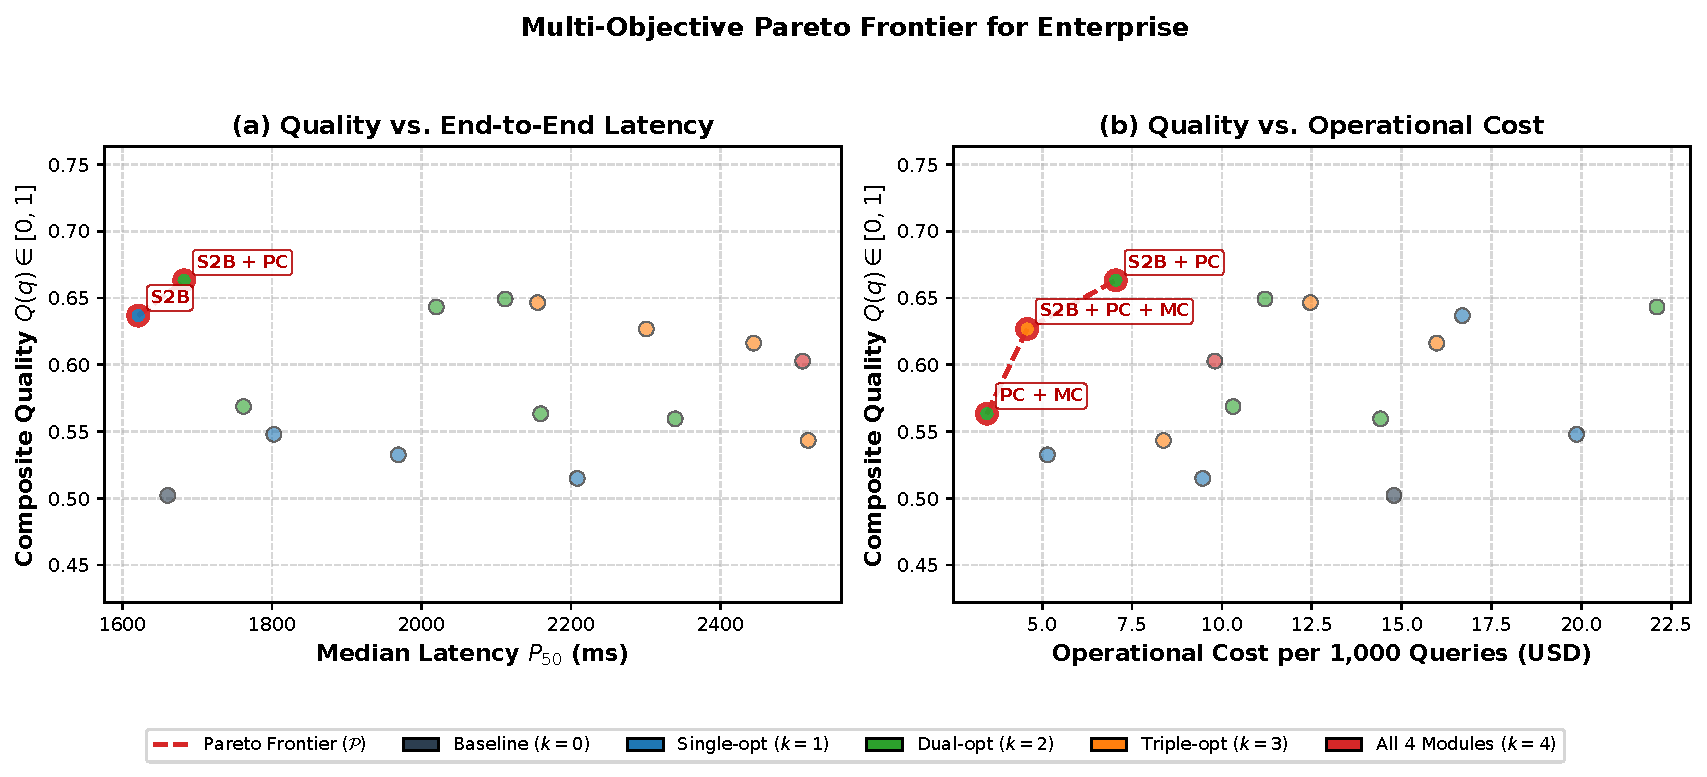
\includegraphics[width=\linewidth]{figures/enterprise/pareto_frontier_enterprise.pdf}
\caption{Empirical Pareto frontier of Composite Quality ($Q$) versus median end-to-end execution latency ($T_{\text{total}}\ P_{50}$) and operational expenditure ($\text{Cost}_{1\text{k}}$) on the unconstrained raw enterprise corpus. Solid lines delineate the non-dominated empirical Pareto frontier across configurations.}
\label{fig:pareto_frontier_enterprise_raw}
\end{figure}
